\documentclass[a4paper, twocolumn]{article}
\usepackage[numbers,sort&compress]{natbib}
\renewcommand{\bibnumfmt}[1]{#1.}
\usepackage[english]{babel}
\usepackage[utf8]{inputenc}
\usepackage{amsmath}
\usepackage{url}
\usepackage{graphicx}
\usepackage[colorinlistoftodos]{todonotes}

\title{RNA Polymerases IV and V: evolution and function}

\author{Carlotta Porcelli, qbp693}

\date{\today}

\begin{document}
\maketitle

\begin{abstract}
Plants have evolved two RNA Polymerases which are not found in other species. RNA Pol IV and Pol V are involved in the RNA-dependent DNA-methylation pathway. 
Pol IV initiates short non-coding RNAs (siRNAs) which are bound to proteins from the Argonaute family. Pol V transcribes long-non-coding RNAs (lncRNAs) which, through  interactions with the AGO-siRNAs complexes, trigger the recruitment of DNA methyltransferase to guide \textit{de novo} cytosine methylation on complementary DNA transcripts. 
Word count: 1700 words.
\end{abstract}

\section{Introduction}
Most of the known non-coding RNAs (ncRNAs) correspond to intergenic sequences or transcripts with unknown functions. In mammals, two of the increasingly known long ncRNAs are \textit{Xist} and \textit{Tsix} which are involved in the regulation of adjacent genes. 
In plants, small-interfering RNAs (siRNAs) guide the process of chromatin modifications. These ncRNAs are generated from specialized machinery responsible for synthesis and action of these small RNAs. Two new polymerases have been observed for the production and functional activity of these siRNAs. In flowering plants, RNA Polymerase IV and RNA Polymerase V are the central enzymes for the RNA-dependent DNA methylation pathway (RdDM). The production of siRNAs transcripts is conducted by RNA Pol IV together with  RNA-dependent RNA polymerase 2 (RDR2). These complexes generate short dsRNAs precursors which are then processed by dicer (DCL) enzymes into 21-24 nucleotides long siRNAs. Downstream to this events, Pol V produces lncRNAs transcripts which, together with the siRNAs association with Argonaute proteins (AGO), guide chromatin modification to homologous DNA sequences \cite{Wierzbicki2009}. 
This report explores the key factors of this RdDM pathway with an insight into evolution and function of RNA Pol IV and RNA Pol V.

\section{The paradox of epigenetic control}
Transcriptional silencing happens most of the time through methylation of CpG islands located in gene promoters. Nevertheless, several tissue-specific genes have CpG islands located downstream of transcription initiation sites. When those regions are methylated elongation is not blocked. 
Plants uniquely use transcription to keep a locus silent; the evolution of specialized RNA Pol IV and V allows transcription of intergenic and non-coding sequences that facilitate heterochromatin formation and silencing of overlapping and adjacent genes. 
The existence of this newly discovered silencing polymerase could explain the paradox of RNA being involved in silencing pathways for the maintenance of transcriptional silencing \cite{Herr118}.  

\section{RNA Polymerase IV}
Pol IV is thought to initiate the RdDM pathway as it physically co-localizes with loci that undergo RdDM and it is essential for 24-nucleotide siRNA biogenesis for the
vast majority of the loci. \cite{Pontes2006}. 

\subsection{The subunits}
Pol IV, as well as Pol II, is composed of 12 subunits. The largest and second largest subunits named NRPD1  and NRPD2 form the catalytic center of the enzyme. The CTD domain lacks the repeating heptad motif found in the CTD of Pol II but it shares with Pol V a single conserved domain Defective Chloroplast and Leaves (DeCL). 
Six of the non-catalytic subunits of Pol IV are found in Pol II as well. The remaining four give functional specificity to the enzyme. They are positioned around the DNA entry and RNA exit channels and surround the catalytic subunits. The 4th and 7th subunits form a complex called 'Stalk' positioned near the RNA exit channel. The 5th and 9th subunits interact with the downstream DNA duplex and form the 'Jaw' complex \cite{ZHOU2015}. The subunits schema is presented in Figure \ref{fig:subunits}.

\subsection{Transcripts and function}
Pol IV is required for the production of 24nt-siRNA in \textit{A. thaliana}  \cite{Zhang130}. These transcripts are generated from both strands and they both lack a poly-A tail. On top of that they also lack a 5' cap. Downstream of the Pol IV activity a RDR2 (RNA-dependent RNA Polymerase 2) is present, it processes the single stranded siRNA into double stranded siRNAs. 

The first step of the biogenesis of the siRNAs is the association of Pol IV with chromatin. This process is mediated by Sawadee Homeodomain Homolog 1 (SHH1) \cite{LAW2013} having a specific role in connection with Pol IV. The Sawadee domain recognizes H3K9 (Histone3-lysine9) methylation and adopts a specific folding that enables the interrgation of the methylation status on H3K9 and H3K4 positions. In \textit{A. thaliana} H3K9 maps on DNA regions enriched with methylation. So SHH1 connects Pol IV with the H3K9 methylation establishing a self-reinforcing loop between repressive chromatin modifications. 
Pol IV transcripts are synthesized into double-stranded RNAs (dsRNAs) by RDR2; this biogenesis is assisted by the chromatin remodeller CHR38, an helicase domain protein. They are subsequently diced into 24-nt siRNAs by the enzyme Dicer-like 3 (DCL3), stabilized by methylation at their 3' ends by Hua Enhancer (HEN1) and loaded into Argonaute (AGO4) effector protein forming the (RNA-induced silencing complex) RISC. 
The whole model of action of Pol IV and Pol V is shown in Figure \ref{fig:model}.

\begin{figure}
	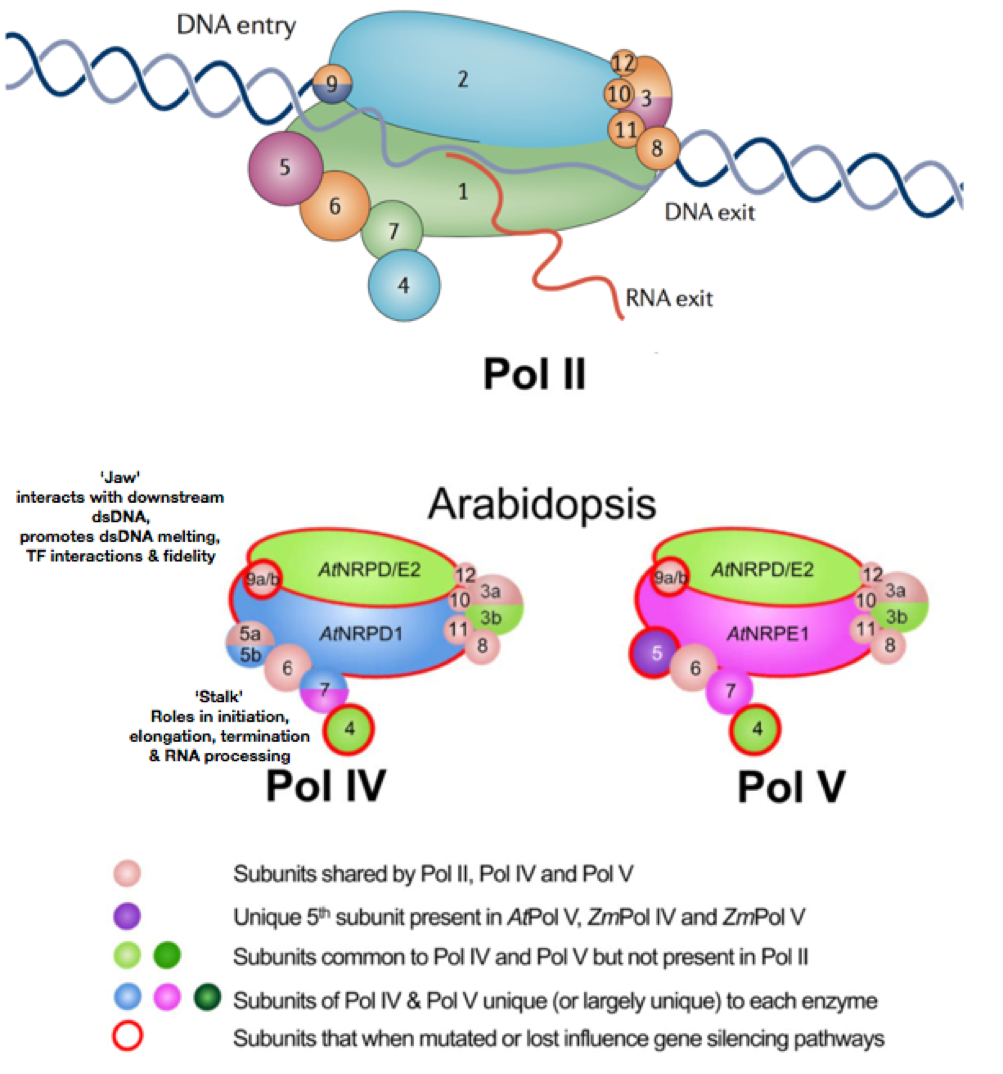
\includegraphics[width=8cm]{my_subunits.png}
	\caption{\textit{Arabidospis thaliana} Pol II, Pol IV and Pol IV subunits schema. Taken from \cite{HAAG2011} and \cite{ZHOU2015}}
	\label{fig:subunits}
\end{figure}

\section{RNA Polymerase V}
Nuclear RNA polymerase V (Pol V) is a multi-subunit plant-specific RNA polymerase with a role in the siRNA-directed DNA methylation (RdDM) pathway and transcriptional gene silencing \cite{ZHOU2015}.

\subsection{The subunits}
Pol V is composed of 12 subunits, half of which are encoded by the same genes as the Pol II homologous subunits \cite{ZHOU2015}. The two largest subunits, namely NRPE1 and NRPE2, arose from independent duplication events and sub-functionalization from their Pol II counterparts. The subunits presented below have been individuated from the  \textit{Arabidopsis thaliana} cauliflower. 
The NRPE1 is characterized by long a C-terminal domain (CTD) of about 700 amino acids. At the C terminus a subdomain rich in glutamine-serine (QS) motifs has been characterized. This domain is preceded by a Defective Chloroplast and Leaves (DeCL) domain with sequence similarities to chloroplast proteins involved in ribosomal RNA processing \cite{HUANG2015}. At the N-terminal of this domain ten repeats of 17 amino acids rich in glycine-tryptophan residues has been identified which coordinates AGO4 slicing of Pol V transcripts and subsequent recruitment of DRM2 methyltransferase.
NRPE1, together with Pol V second largest subunit NRPE2, form the catalytic subunits comparable to NRPB1 and NRPB2 of Pol II. 
The other 10 subunits do not have catalytic activity, and they characterize Pol V functions. Subunits 3, 4, 5  and 7 cluster on the 'leading face' of the polymerase enzyme and surround the catalytic center, the DNA entry and the RNA exit channels.
As well as in Pol IV, the 'Stalk' and 'Jaw' complexes are found in Pol V \cite{HAAG2011}. The subunits schema is presented in Figure \ref{fig:subunits}.

\subsection{Transcripts and function}
A characterized region of the genome, rich in DNA methylation at intergenic loci, has been analyzed by Wierbicki et al. \cite{wierzbick1} to elucidate the role of Pol V in targeting chromatin modifications. 
The chromomere on the northern arm of \textit{A. thaliana}, on chromosome 4, is rich in heterocromatic repeats and transposons. This area has been investigated for Intergenic non-coding regions (IGN). A set of six IGN transcripts has been identified to be reduced or absent in \textit{pol v} mutants. These transcripts can be up to 200 nt long and therefore are defined as lncRNAs (long non-coding RNAs). Their initiation can happen in multiple adjacent sites. They lack poly-A tails and their 5' ends are a mixture of 5' triphosphates and monophosphates. 
The recruitment of Pol V to chromatin IGN producing loci has been shown to depend on two components: Defecting in RNA-dependent DNA methylation 1 (DRD1) and Defective in Meristem silencing 3 (DMS3) \cite{wierzbick1}. Moreover a new component, RDM1, has been identified to stably associate with DRD1 and DMS3. These three components form a complex termed DDR that facilitate Pol V association with chromatin via a direct interaction  \cite{LAW2010}. On top of this, other two methyl-DNA binding proteins (SU(VAR)3-9 homolog 2: SUVH2 and SUVH9) have been found interacting with the DDR complex \cite{Johnson2014} and are required for Pol V chromatin association. These interactions lead to a model in which Pol V recruitment depends on pre-existing DNA methylation bound by  SUVH2 and SUVH9 which then interact with the DDR complex that promotes Pol V association.
The siRNAs produced by Pol IV, associated with AGO4 proteins, guide cytosine methylation through base-pairing interaction with the nascent lncRNAs transcripts of Pol V. \cite{Wierzbicki2009} This interaction facilitates the recruitment of Domains Rearranged Methyltransferase 2 (DRM2) and Chromatin Remodelling 28 and 28 (CHR27 / CHR28) that regulate the activity of Pol V and facilitate \textit{de novo} DNA methylation.
As shown in \cite{LAHMY2016} in the C-terminal domain of Pol V largest subunit NRPE1, and its associated factor SPT5L (a Pol V auxiliary protein), is present a conserved domain of glycine-tryptophan/tryptophan-glycine (GW/WG) region. Its function is shown to be essential to hook AGO proteins and facilitate the bond of their siRNA sequences to the DNA chromatin targets. These motifs recruit a massive amount of AGO4 siRNA loaded complexes to their site of action. The increase of local concentration of AGO4 is a consequence of the stabilization of Pol V to the DNA strand. The model proposed sees, firstly, Pol V proceeding through transcription elongation, followed by the AGO4 interacting with the lncRNAs Pol V-transcripts generating an intermediate complex that would serve for the transfer of AGO4 to the DNA template. At this stage AGO4 recruits  DNA (cytosine-5)-methyltransferase (DRM2) to the opposite DNA strand to trigger DNA methylation.
The whole model of action of Pol IV and Pol V is shown in Figure \ref{fig:model}.

\begin{figure}
	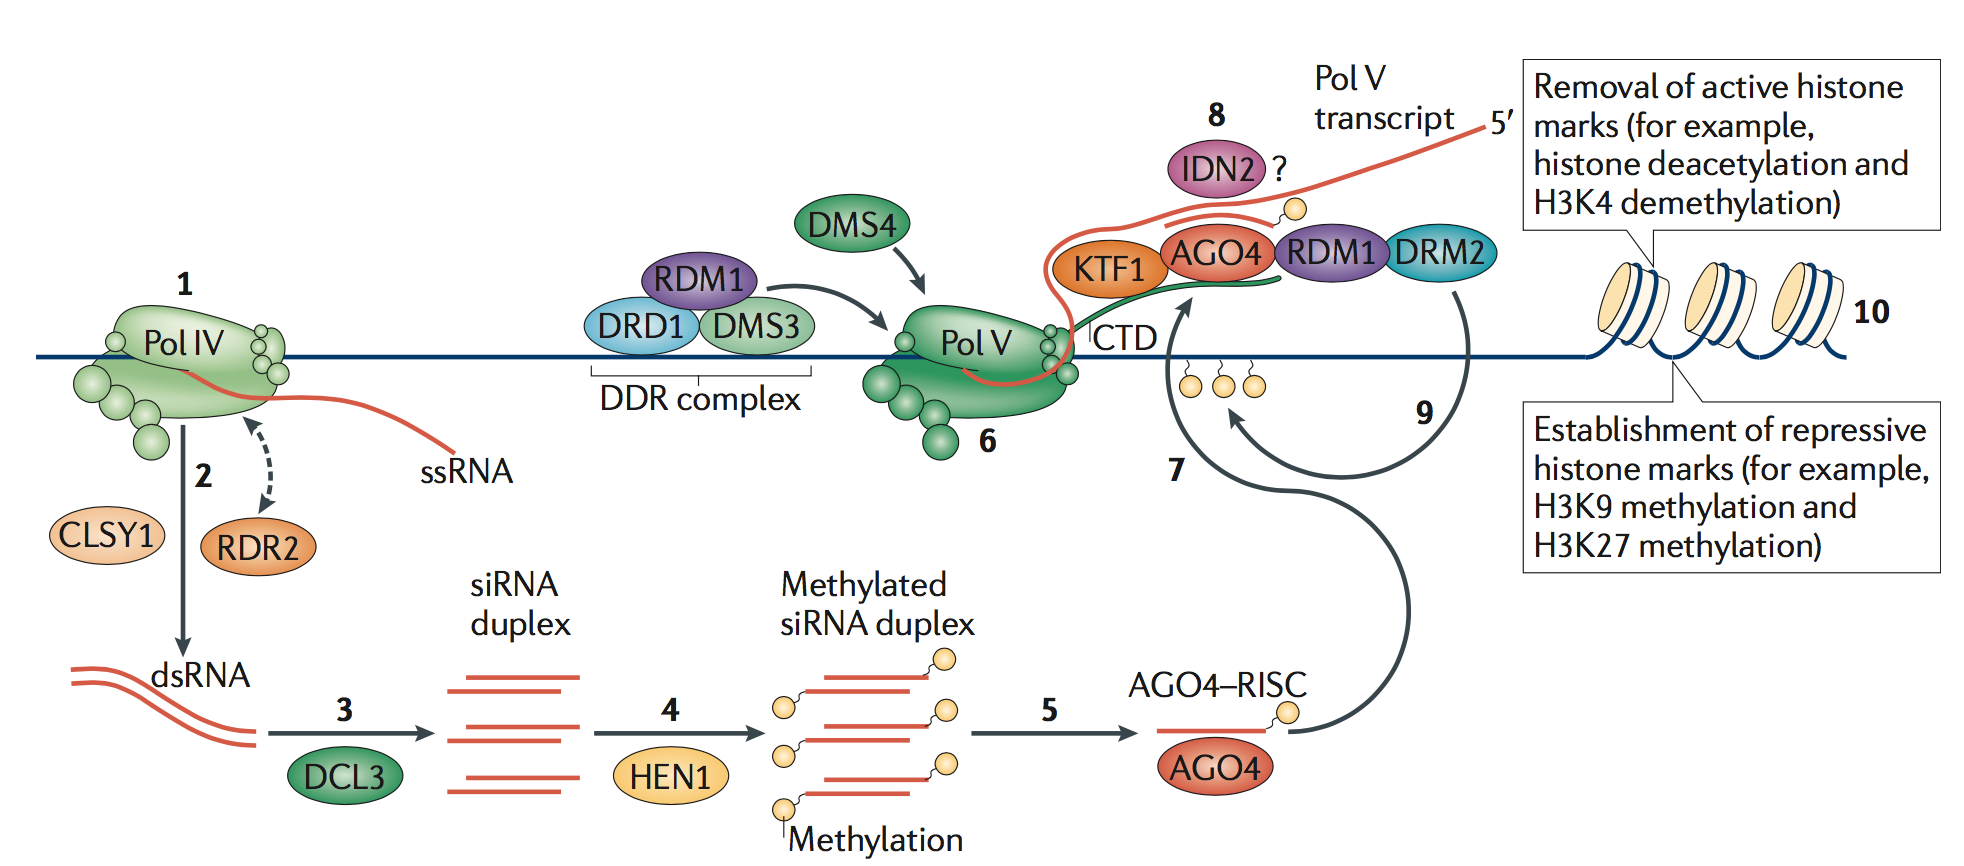
\includegraphics[width=9cm]{complete_process.png}
	\caption{Model for the RNA-directed DNA methylation pathway in \textit{Arabidospis thaliana}. Taken from \cite{HAAG2011}}
	\label{fig:model}
\end{figure}

\section{Future outlook}
It is still unclear which templates the two polymerases use \textit{in vivo} and how the transcription is regulated in order not to produce aberrant non-coding RNAs. 
Further studies need to be conducted to investigate both the transcription initiation and the role of the RNA primers in that process and the termination steps. 

\subsection{Pol IV}
The recruitment of the Pol IV to targets different from H3K9 methylated sites is still unclear. Moreover the SHH1 factor, needed for Pol IV association with chromatin, recognizes H3K9 methylation and unmethylated H3K4 on the loci where the Pol IV will be recruited downstream. \cite{LAW2013} It is still not clear how the histone methylation are initially established in the specific loci.

\subsection{Pol V}
The association of Pol V to the chromatin seems to involve more factors than the few ones discussed in this work, as shown in \cite{STROUD2012}. Nevertheless  their specific function is still unclear and could be elucidated in further studies. 
Not much is known on the nature and function of the IGN Pol V transcripts and this could be a case of future studies as well. 

\bibliography{essay_bibliography}
\bibliographystyle{currbiol}

\end{document}